\documentclass[10pt]{article}
\usepackage{icmlko}

\icmlmeta{IP 파운데이션 월드모델}{293}{만나는 것은 같은 작품이다}{별칭 사전이 만화↔웹툰을 1건에서 175건으로 열었다 --- 그런데 152건이 같은 작품이고 lab 은 이미 그걸 걸러 놓았다}

\begin{document}

\twocolumn[
\icmlheader

\begin{abstract}
노트 291이 ``도메인끼리 이름으로 안 만난다''로 끝나면서 별칭 사전을 남은
것으로 적었다. 조사했다(병렬 에이전트). \textbf{웹툰↔애니에서는 별칭이
소용없다} --- 둘 다 이미 한국어라 표기 문제가 아니고, 병목은 모집단이다
(웹툰 2,817편 중 라프텔에 애니가 있는 게 원래 십수 편). 천장이 14$\sim$20건
이고 그 증가분도 별칭이 아니라 \emph{시즌 접미사 정리}에서 나온다.
\textbf{그런데 만화↔웹툰은 다르다} --- \texttt{cache\_manga\_kr} 에 한글 원제가
있어 \textbf{1건 $\to$ 175건}이 된다. 여기서 멈추지 않고 그 175건이 무엇인지
봤다. \textbf{만화가 웹툰보다 먼저 시작한 것은 23건(0.8\%)}이고 나머지
\textbf{152건은 같은 작품이 두 곳에 있는 것}이다 --- AniList 의 MANGA 포맷이
한국 웹툰을 포함하기 때문이다. 그리고 \textbf{lab 의 만화 도메인은 그 전부를
이미 제외하고 있다}: 만화 레코드는 JP 1,789 · KR 556 · CN 55 인데 \textbf{lab
도메인은 JP 1,789 뿐}이다. 웹툰과 붙는 것은 전부 KR 556 안에 있다. 그래서
\textbf{웹툰 유보 $\times$ 만화 학습 중복 쌍이 0개}다 --- 중복 누출이 없다.
\textbf{도메인이 만나는 자리는 대개 전이가 아니라 중복이고, 이 실험실은 그걸
이미 걸러 놓았다.} 진짜 크로스 IP 23건은 웹툰의 0.8\% 라 검출 문턱
0.046 근처도 못 간다.
\end{abstract}
]

\section{별칭 사전을 실제로 세어 봤다}

노트 291이 열한 도메인이 이름으로 안 만난다는 것을 재고(웹툰↔애니 10건 ·
만화↔게임 1건), 원인을 ``표기가 다르다''로 적었다. 별칭 사전이 그걸 고칠 수
있는지 재료를 세었다.

\begin{center}\small
\begin{tabular}{lr}
\hline
재료 & \\
\hline
세계애니 \texttt{synonyms} 중 한글 포함 & 85 / 7,169 (\textbf{1.2\%}) \\
\texttt{anime\_match.json} 다리 & 87건 (그중 51 해소) \\
\texttt{cache\_manga\_kr} 한글 원제 & 1,250 (만화 556건 덮음) \\
모바일 \texttt{bundleId} IP 토큰 수율 & \textbf{0.3\%} \\
\hline
\end{tabular}
\end{center}

\paragraph{웹툰↔애니에서는 별칭이 소용없다} 누적 실험 결과 9 $\to$ 14 $\to$
15건인데, 증가분의 대부분(9$\to$14)이 \emph{별칭이 아니라 시즌 · 괄호 접미사
정리}에서 나온다. \texttt{anime\_match}(87건)와 세계애니 한글 별칭(85개)을
통째로 넣어도 \textbf{증가 0건}이다. 이유는 명확하다 --- \textbf{웹툰과
라프텔은 이미 둘 다 한국어다.} 표기가 문제가 아니라 \textbf{모집단이 안
겹친다}(웹툰 2,817편 중 라프텔에 애니가 있는 작품이 원래 십수 편).
\textbf{노트 291의 진단이 이 쌍에서는 틀렸다.}

\section{만화↔웹툰은 1건에서 175건}

\begin{figure*}[t]
\centering
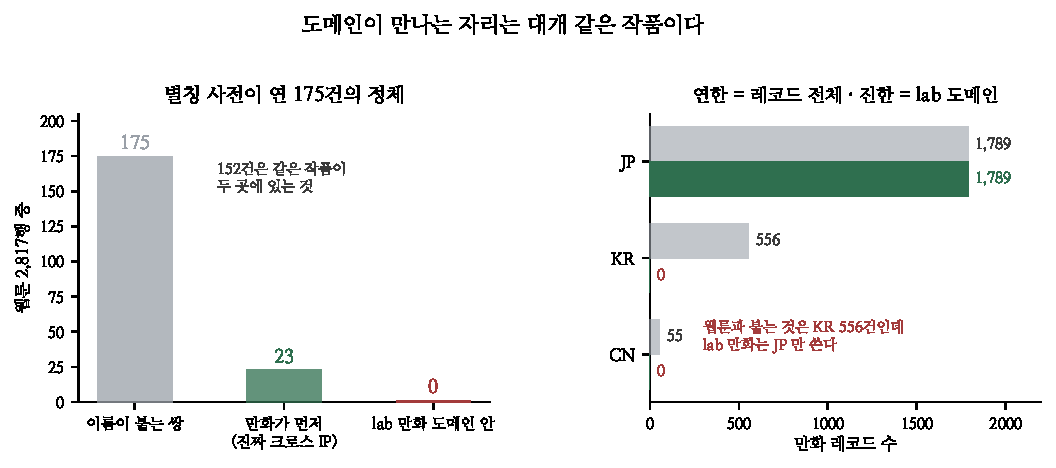
\includegraphics[width=\textwidth]{figs/same.pdf}
\caption{왼쪽 --- 별칭 사전이 연 175건을 갈라 본 것. 오른쪽 --- 만화 레코드의
국가 분포와 lab 만화 도메인.}
\end{figure*}

만화는 다르다. \texttt{manga\_records} 의 \texttt{title} 이 romaji 뿐인데
(\texttt{Kimetsu no Yaiba}) \texttt{cache\_manga\_kr} 에 한글 원제가 있다.
붙이면 \textbf{만화↔웹툰이 1건 $\to$ 175건}이다.

\textbf{여기서 멈추면 안 된다}(노트 133). 그 175건이 무엇인지 봤다.

\begin{center}\small
\begin{tabular}{lr}
\hline
웹툰 2,817행 중 & \\
\hline
만화와 이름이 붙는 쌍 & 175 \\
\textbf{만화가 먼저 시작한 것} & \textbf{23} (0.8\%) \\
나머지 & 152 \\
\hline
\end{tabular}
\end{center}

\textbf{152건은 웹툰이 먼저다.} AniList 의 \texttt{MANGA} 포맷이 한국
웹툰(만화)을 포함하기 때문이다 --- 같은 작품이 두 도메인에 있는 것이지 다른
IP 가 만난 것이 아니다.

\section{lab 은 이미 걸러 놓았다}

같은 작품이 한쪽은 학습, 한쪽은 채점이면 \textbf{중복 누출}이다. 셌다.

\begin{center}\small
\begin{tabular}{lrr}
\hline
& 레코드 전체 & lab 만화 도메인 \\
\hline
JP & 1,789 & \textbf{1,789} \\
KR & 556 & \textbf{0} \\
CN & 55 & \textbf{0} \\
\hline
\end{tabular}
\end{center}

\textbf{lab 의 만화 도메인은 일본 것만 쓴다.} 웹툰과 붙는 175건은 전부 제외된
KR 556 안에 있다. 그래서

\begin{center}\small
\textbf{웹툰 유보 $\times$ 만화 학습 중복 쌍 ${=}$ 0개}
\end{center}

이다. \textbf{누출이 없다.} 그 제외가 의도였는지 우연이었는지는 이 노트에서
확인 안 했지만, 결과는 옳다.

\paragraph{그리고 그래서 크로스 링크도 0이다} 같은 제외가 \emph{쓸 수 있는}
링크도 같이 없앤다. 진짜 크로스 IP 23건도 KR 안에 있어 lab 의 만화 도메인엔
없다. \textbf{누출을 막는 벽과 전이를 막는 벽이 같은 벽이다.}

\section{그리고 라벨은 어차피 못 쓴다}

설령 링크가 있어도 \textbf{만화의 라벨은 못 쓴다.} \texttt{y\_popularity} 는
AniList 의 \textbf{지금 긁은 스냅샷}이고(\texttt{label\_basis} 가 2,400건
전부 비어 있다) 노트 224가 \texttt{kitsu\_rating} · \texttt{kitsu\_rank} 를
막은 것과 같은 이유로 \textbf{사후}다 --- 웹툰이 연재를 시작하는 시점에 그
만화의 현재 인기는 존재하지 않는다.

쓸 수 있는 것은 라벨이 아니라 \textbf{존재와 시점}이다: ``이 IP 가 웹툰 이전에
만화로 있었나.'' 그게 23건이고 웹툰의 \textbf{0.8\%} 다. 노트 274가 잰 웹툰의
검출 문턱이 0.046 인데, 행의 0.8\% 만 건드리는 축이 그만큼을 낼 수는 없다.

\paragraph{남은 것}
\begin{center}\small
\begin{tabular}{ll}
\hline
갈래 & 왜 \\
\hline
만화 KR 556 을 도메인으로 & 웹툰과 중복이라 안 된다 \\
회사 축 & 게임↔모바일 59개는 아직 안 재 봤다 \\
팝업 허브 & 노트 291의 조인은 여전히 유효 \\
하네스에서 재기 & 분해능이 다른 유일한 자리 \\
\hline
\end{tabular}
\end{center}

\paragraph{규약} \textbf{도메인이 만나면 전이인지 중복인지 먼저 가른다.}
``만화↔웹툰 175건''은 얼핏 크로스 도메인 전이의 재료로 보이지만 152건이 같은
작품이었다. 그리고 \textbf{누출을 막는 설계는 전이도 같이 막는다} ---
lab 의 만화가 일본 것만 쓰는 것이 중복 누출을 0으로 만들고 동시에 크로스
링크도 0으로 만든다. \textbf{둘 중 하나만 고를 수는 없다.}

\end{document}
